\section{Week - 13-18.05.2026 - Fourier Transform and PDEs}

\begin{itemize}
    \item If $x \in [0,L]$: We use the \textbf{Fourier series decomposition}.
    \item If $x \in \R$: We use the \textbf{Fourier transform} in $x$.
\end{itemize}

\begin{recall}
    If $f : \R \rightarrow \C$, the Fourier transform is defined as:
    $$ \mathcal{F}[f](a) = \hat{f}(a) = \frac{1}{\sqrt{2\pi}} \int_{-\infty}^{+\infty} e^{-iax} f(x) \dd x $$
    (provided $\int_{-\infty}^{+\infty} |f(x)| \dd x < +\infty$).
\end{recall}

\textbf{Important properties:}
\begin{align*}
    \mathcal{F}\left[\frac{\partial f}{\partial x}\right](a) &= ia \mathcal{F}[f](a), \\[1ex]
    \mathcal{F}[f](a) \cdot \mathcal{F}[g](a) &= \frac{1}{\sqrt{2\pi}} \mathcal{F}[f * g](a)
\end{align*}

\subsection{The Heat Equation}

Consider the inhomogeneous heat equation:
\begin{equation}
\begin{cases}
    \displaystyle \frac{\partial u}{\partial t} - \frac{\partial^2 u}{\partial x^2} = f(x,t), & x \in \R, t>0, \\[2ex]
    u(x,0) = u_0(x)
\end{cases}
\end{equation}

(We assume that $\int_{-\infty}^{+\infty} |u_0(x)| \dd x < +\infty$ and $\int_{-\infty}^{+\infty} |f(x,t)| \dd x < +\infty$ so that we can appropriately apply the Fourier transform).

Applying the Fourier transform in $x$:
\begin{align*}
    \hat{u}(a,t) &= \frac{1}{\sqrt{2\pi}} \int_{-\infty}^{+\infty} e^{-iax} u(x,t) \dd x \\
    \hat{u}_0(a) &= \frac{1}{\sqrt{2\pi}} \int_{-\infty}^{+\infty} e^{-iax} u_0(x) \dd x \\
    \hat{f}(a,t) &= \frac{1}{\sqrt{2\pi}} \int_{-\infty}^{+\infty} e^{-iax} f(x,t) \dd x
\end{align*}

Then the PDE becomes:
$$ \frac{\partial u}{\partial t} - \frac{\partial^2 u}{\partial x^2} = f \implies \mathcal{F}\left[ \frac{\partial u}{\partial t} - \frac{\partial^2 u}{\partial x^2} \right](a,t) = \hat{f}(a,t) $$

This yields the system:
\begin{equation*}
\begin{cases}
    \displaystyle \frac{\partial \hat{u}}{\partial t}(a,t) + a^2 \hat{u}(a,t) = \hat{f}(a,t) \\[2ex]
    \hat{u}(a,0) = \hat{u}_0(a)
\end{cases}
\end{equation*}

For each frequency $a \in \R$, this is a first-order \textbf{ODE in time}! We can solve it (e.g., using the Laplace transform in $t$, or an integrating factor).

\textbf{Solution:}
\begin{equation}
    \hat{u}(a,t) = e^{-a^2t}\hat{u}_0(a) + \int_0^t e^{-a^2(t-s)}\hat{f}(a,s) \dd s
\end{equation}

We need to apply the \textit{inverse Fourier transform} to get an expression for $u(x,t)$. 

\begin{recall}
    The Fourier transform of a Gaussian is a Gaussian:
    $$ \mathcal{F}\left[ e^{-\frac{x^2}{2}} \right](a) = e^{-a^2/2} $$
    Also, recall the rescaling property: 
    $$ \mathcal{F}[f(\lambda x)](a) = \frac{1}{|\lambda|}\mathcal{F}[f]\left(\frac{a}{\lambda}\right) $$
\end{recall}

Using this, we can invert $e^{-a^2t}$:
$$ e^{-a^2t} = e^{-\frac{(\sqrt{2t} \cdot a)^2}{2}} = \frac{1}{\sqrt{2t}} \mathcal{F}\left[ e^{-\frac{1}{2} \left( \frac{x}{\sqrt{2t}} \right)^2} \right](a) = \mathcal{F}\left[ \frac{1}{\sqrt{2t}} e^{-\frac{x^2}{4t}} \right](a) $$

Going back to our ODE solution (2):
$$ \hat{u}(a,t) = \mathcal{F}\left[ \frac{1}{\sqrt{2t}} e^{-\frac{x^2}{4t}} \right](a) \cdot \mathcal{F}[u_0](a) + \int_0^t \mathcal{F}\left[ \frac{1}{\sqrt{2(t-s)}} e^{-\frac{x^2}{4(t-s)}} \right](a) \cdot \mathcal{F}[f(\cdot,s)](a) \dd s $$

Inverting (and using the property about convolutions):
\begin{equation}
\begin{aligned}
    u(x,t) &= \frac{1}{\sqrt{4\pi t}} \int_{-\infty}^{+\infty} e^{-\frac{(x-y)^2}{4t}} u_0(y) \dd y \\
    &\quad + \int_0^t \int_{-\infty}^{+\infty} \frac{1}{\sqrt{4\pi (t-s)}} e^{-\frac{(x-y)^2}{4(t-s)}} f(y,s) \dd y \, \dd s
\end{aligned}
\end{equation}

\textbf{Special case:} When $f = 0$, we just have the first term:
$$ u(x,t) = \frac{1}{\sqrt{4\pi t}} \int_{-\infty}^{+\infty} e^{-\frac{(x-y)^2}{4t}} u_0(y) \dd y $$

\begin{center}
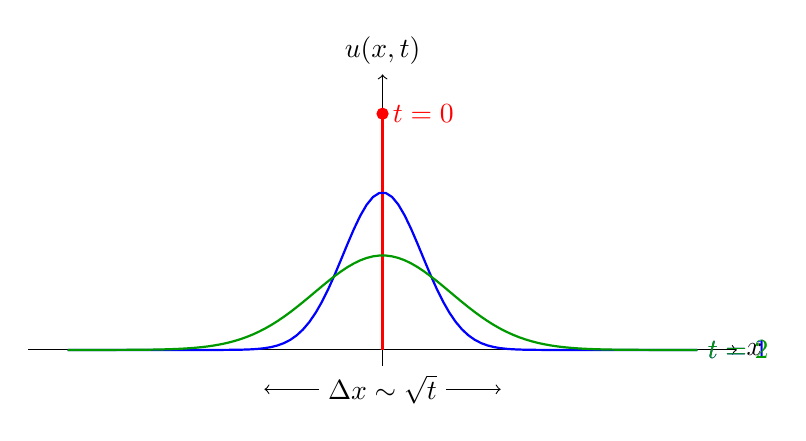
\begin{tikzpicture}[domain=-4:4, samples=100, scale=1]
    % Axes
    \draw[->] (-4.5,0) -- (4.5,0) node[right] {$x$};
    \draw[->] (0,-0.2) -- (0,3.5) node[above] {$u(x,t)$};
    
    % t=0 (Dirac delta approximation)
    \draw[color=red, thick] (0,0) -- (0,3) node[right] {$t=0$};
    \filldraw[red] (0,3) circle (2pt);
    
    % t=1 Gaussian
    \draw[color=blue, thick] plot (\x, {2*exp(-(\x*\x)/0.5)}) node[right] {$t=1$};
    
    % t=2 Gaussian
    \draw[color=green!60!black, thick] plot (\x, {1.2*exp(-(\x*\x)/1.5)}) node[right] {$t=2$};
    
    % Delta x scaling
    \draw[<->] (-1.5, -0.5) -- (1.5, -0.5) node[midway, fill=white] {$\Delta x \sim \sqrt{t}$};
\end{tikzpicture}
\end{center}

\begin{theorem}[Duhamel's Principle]
If $P[u_0](x,t)$ is the above integral expression for the homogeneous case, then the solution in the case when $f \neq 0$ is given by:
$$ u(x,t) = P[u_0](x,t) + \int_0^t P[f(\cdot, s)](x, t-s) \dd s $$
\end{theorem}

\subsection{Another Example: Wave Equation}

\begin{equation}
\begin{cases}
    \displaystyle \frac{\partial^2 u}{\partial t^2} - \frac{\partial^2 u}{\partial x^2} = f(x,t) & \text{for } x \in \R, t > 0 \\
    u(x,0) = u_0(x) \\
    \displaystyle \frac{\partial u}{\partial t}(x,0) = u_1(x)
\end{cases}
\end{equation}
(We set $c=1$ for simplicity).

Apply a Fourier transform in $x$:
$$ \hat{u}(a,t) = \frac{1}{\sqrt{2\pi}} \int_{-\infty}^{+\infty} e^{-iax} u(x,t) \dd x $$
and similarly for $\hat{f}(a,t)$, $\hat{u}_0(a)$, and $\hat{u}_1(a)$.

Then, noting that $\mathcal{F}\left[\frac{\partial^2 u}{\partial x^2}\right] = (ia)^2 \hat{u} = -a^2 \hat{u}$, we get:
\begin{equation}
\begin{cases}
    \displaystyle \frac{\partial^2 \hat{u}}{\partial t^2}(a,t) + a^2 \hat{u}(a,t) = \hat{f}(a,t) \\[2ex]
    \hat{u}(a,0) = \hat{u}_0(a) \\[1ex]
    \displaystyle \frac{\partial \hat{u}}{\partial t}(a,0) = \hat{u}_1(a)
\end{cases}
\end{equation}

Solution (using Laplace transform in $t$, or variation of parameters):
$$ \hat{u}(a,t) = \cos(at) \hat{u}_0(a) + \frac{1}{a}\sin(at) \hat{u}_1(a) + \int_0^t \frac{1}{a} \sin(a(t-s)) \hat{f}(a,s) \dd s $$

We need to invert the Fourier transform; this is a bit trickier than before.

\begin{itemize}
    \item For the $\cos(at)\hat{u}_0(a)$ term, recall the translation property:
    $$ \mathcal{F}[h(x+c)](a) = e^{iac} \mathcal{F}[h(x)](a) $$
    So:
    \begin{align*}
        \hat{u}_0(a) \cdot \cos(at) &= \hat{u}_0(a) \frac{e^{iat} + e^{-iat}}{2} \\
        &= \frac{1}{2} \mathcal{F}[u_0(x+t) + u_0(x-t)](a)
    \end{align*}

    \item For the $\frac{1}{a}\sin(at) \hat{u}_1(a)$ term, we use the fact that if:
    $$ h(x) = \begin{cases} 1, & -1 \leq x \leq 1 \\ 0, & \text{else} \end{cases} $$
\end{itemize}

\begin{center}
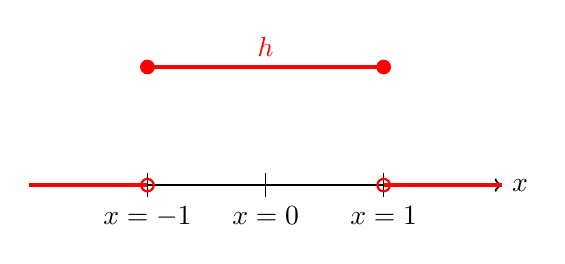
\begin{tikzpicture}[scale=1.5]
    % Axis
    \draw[->, thick] (-2,0) -- (2,0) node[right] {$x$};
    
    % Ticks
    \draw (-1, 0.1) -- (-1, -0.1) node[below] {$x=-1$};
    \draw (0, 0.1) -- (0, -0.1) node[below] {$x=0$};
    \draw (1, 0.1) -- (1, -0.1) node[below] {$x=1$};
    
    % Function line
    \draw[red, very thick] (-2,0) -- (-1,0);
    \draw[red, very thick] (1,0) -- (2,0);
    \draw[red, very thick] (-1,1) -- (1,1) node[midway, above] {$h$};
    
    % Circles
    \draw[red, thick] (-1,0) circle (1.5pt);
    \draw[red, thick] (1,0) circle (1.5pt);
    \filldraw[red, thick] (-1,1) circle (1.5pt);
    \filldraw[red, thick] (1,1) circle (1.5pt);
\end{tikzpicture}
\end{center}

Then $\hat{h}(a) = \sqrt{\frac{2}{\pi}} \cdot \frac{\sin(a)}{a}$ (Exercise).

Using the rescaling property $\mathcal{F}[h(\lambda x)](a) = \frac{1}{|\lambda|} \mathcal{F}[h]\left(\frac{a}{\lambda}\right)$ and the fact that 
$$ h_t(x) = \begin{cases} 1, & -t \leq x \leq t \\ 0, & \text{else} \end{cases} $$
is just $h_t(x) = h(x/t)$, we compute:
$$ \hat{h}_t(a) = \sqrt{\frac{2}{\pi}} \cdot \frac{\sin(at)}{a} $$

Therefore:
\begin{align*}
    \hat{u}_1(a) \cdot \frac{\sin(at)}{a} &= \mathcal{F}[u_1](a) \cdot \sqrt{\frac{\pi}{2}} \cdot \mathcal{F}[h_t](a) \\
    &= \frac{1}{2} \mathcal{F}[u_1 * h_t](a)
\end{align*}

Evaluating the convolution:
$$ (u_1 * h_t)(x) = \int_{-\infty}^{+\infty} h_t(x-y) u_1(y) \dd y = \int_{x-t}^{x+t} u_1(y) \dd y $$

\begin{verification}[Correction of D'Alembert's Formula]
In the original handwritten notes, the integral over the source term $f(y,s)$ is incorrectly written as $\int_{x-t}^{x+t} f(y,s) \dd y \dd s$. 

By Duhamel's Principle, the source term is treated as a series of initial velocity profiles $f(y,s)$ injected at time $s$. The domain of dependence for the perturbation at $(x,t)$ originating from time $s$ is governed by the time elapsed, which is $(t-s)$, not $t$. Therefore, the spatial bounds for the integral at time $s$ must be $[x-(t-s), x+(t-s)]$. We correct this below.
\end{verification}

So, overall (D'Alembert's Formula):
\begin{formula}[D'Alembert's Formula]
\begin{equation}
    u(x,t) = \frac{1}{2}\Big(u_0(x+t) + u_0(x-t)\Big) + \frac{1}{2} \int_{x-t}^{x+t} u_1(y) \dd y + \frac{1}{2} \int_0^t \int_{x-(t-s)}^{x+(t-s)} f(y,s) \dd y \, \dd s
\end{equation}
\end{formula}

\textbf{Finite speed of propagation:}
The value of $u(x,t)$ depends only on the value of $f$ in the shaded light-cone region and the value of $(u_0, u_1)$ on the base segment.

\begin{center}
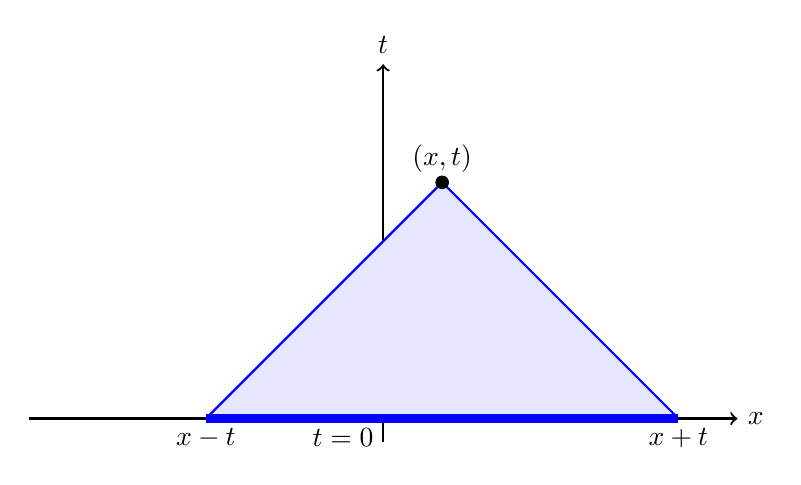
\begin{tikzpicture}[scale=1.5]
    % Axes
    \draw[->, thick] (-3,0) -- (3,0) node[right] {$x$};
    \draw[->, thick] (0,-0.2) -- (0,3) node[above] {$t$};
    
    % Cone coordinates
    \coordinate (Apex) at (0.5, 2);
    \coordinate (LeftBase) at (-1.5, 0);
    \coordinate (RightBase) at (2.5, 0);
    
    % Light cone
    \fill[blue!10] (Apex) -- (LeftBase) -- (RightBase) -- cycle;
    \draw[blue, thick] (LeftBase) -- (Apex) -- (RightBase);
    
    % Base segment
    \draw[blue, line width=3pt] (LeftBase) -- (RightBase);
    
    % Labels
    \filldraw (Apex) circle (1.5pt) node[above] {$(x,t)$};
    \node[below] at (LeftBase) {$x-t$};
    \node[below] at (RightBase) {$x+t$};
    \node[below left] at (0,0) {$t=0$};
\end{tikzpicture}
\end{center}

\newpage
\subsection{The Schrödinger Equation}

Suppose that $u : \R \times (0, +\infty) \rightarrow \C$ solves the following equation:
\begin{equation}
    i \frac{\partial u}{\partial t}(x,t) + \frac{\partial^2 u}{\partial x^2}(x,t) - V(x,t)u(x,t) = 0 \quad \text{for } t>0, x \in \R
\end{equation}

This is the Schrödinger equation with potential $V$.

\begin{itemize}
    \item The potential is always assumed to be real-valued (i.e. $V(x,t) \in \R \;\forall x,t$).
    \item The solution $u$ is necessarily complex-valued in view of the presence of $i$ in the equation.
    \item \textbf{Physical interpretation:} The above equation describes the evolution of a quantum particle moving under the influence of a (classical) potential $V(x,t)$.
\end{itemize}

The quantity $\int_a^b |u(x,t)|^2 \dd x$ is the probability that the particle at time $t$ is in the interval $a \leq x \leq b$. In order for the above ``probabilistic'' interpretation to make sense, we must have:
$$ \int_{-\infty}^{+\infty} |u(x,t)|^2 \dd x = 1 \quad \text{for all times.} $$

In particular, $\int_{-\infty}^{+\infty} |u(x,t)|^2 \dd x$ must be \textbf{constant} in $t$ for solutions $u$ to (1). 

\begin{proofbox}[Proof that $\int_{-\infty}^{+\infty} |u(x,t)|^2 \dd x$ is conserved if $u, \frac{\partial u}{\partial x} \rightarrow 0$ as $x \to \pm\infty$]

\begin{align*}
    \frac{\partial}{\partial t} \int_{-\infty}^{+\infty} |u(x,t)|^2 \dd x &= \frac{\partial}{\partial t} \int_{-\infty}^{+\infty} u(x,t) \cdot \overline{u(x,t)} \dd x \\
    &= \int_{-\infty}^{+\infty} \left( \frac{\partial u}{\partial t} \overline{u} + u \overline{\frac{\partial u}{\partial t}} \right) \dd x \\
    &= \int_{-\infty}^{+\infty} 2 \Re \left\{ \frac{\partial u}{\partial t} \overline{u} \right\} \dd x \tag{A}
\end{align*}

From the equation $i \frac{\partial u}{\partial t} + \frac{\partial^2 u}{\partial x^2} - Vu = 0$, we have $\frac{\partial u}{\partial t} = i\frac{\partial^2 u}{\partial x^2} - iVu$. Substituting this into (A):
\begin{align*}
    \text{(A)} &= \int_{-\infty}^{+\infty} 2 \Re \left\{ \left( i\frac{\partial^2 u}{\partial x^2} - iVu \right) \overline{u} \right\} \dd x \\
    &= \int_{-\infty}^{+\infty} 2 \Re \left\{ i \frac{\partial^2 u}{\partial x^2} \overline{u} - i V |u|^2 \right\} \dd x
\end{align*}

Since $V(x,t)$ and $|u(x,t)|^2$ are real-valued, the term $-iV|u|^2$ is purely imaginary. Therefore, its real part is zero: $\Re \{ -iV|u|^2 \} = 0$.
Returning to the integral:
$$ = 2 \int_{-\infty}^{+\infty} \Re \left\{ i \frac{\partial^2 u}{\partial x^2} \overline{u} \right\} \dd x $$

Integrating by parts:
$$ = 2 \Re \left\{ \left[ i \frac{\partial u}{\partial x} \overline{u} \right]_{x=-\infty}^{+\infty} - \int_{-\infty}^{+\infty} i \frac{\partial u}{\partial x} \frac{\partial \overline{u}}{\partial x} \dd x \right\} $$

If $u(x,t), \frac{\partial u}{\partial x}(x,t) \rightarrow 0$ as $x \rightarrow \pm\infty$ (a reasonable assumption for a ``localized'' particle), then the boundary terms vanish, and the above is:
$$ = -2 \int_{-\infty}^{+\infty} \Re \left\{ i \frac{\partial u}{\partial x} \frac{\partial \overline{u}}{\partial x} \right\} \dd x $$

But $i \frac{\partial u}{\partial x} \frac{\partial \overline{u}}{\partial x} = i \left| \frac{\partial u}{\partial x} \right|^2$ is purely imaginary, so its real part is $0$. 
Thus, the derivative is $0$, and probability is conserved.
\end{proofbox}

\textbf{Initial Value Problem for the (inhomogeneous) Schrödinger equation:}
\begin{equation}
\begin{cases}
    i\frac{\partial u}{\partial t}(x,t) + \frac{\partial^2 u}{\partial x^2}(x,t) - V(x,t)u(x,t) = F(x,t) & \text{for } t>0, x \in \R \\
    u(x,0) = u_0(x)
\end{cases}
\end{equation}

\textbf{Uniqueness of solutions:}
If $u_1, u_2$ are solutions, then $w = u_1 - u_2$ solves the homogeneous system:
$$ \begin{cases}
    i\frac{\partial w}{\partial t} + \frac{\partial^2 w}{\partial x^2} - V w = 0 \\
    w(x,0) = 0
\end{cases} $$
By the conservation law proved above:
$$ \forall t > 0 : \int_{-\infty}^{+\infty} |w(x,t)|^2 \dd x = \dots = \int_{-\infty}^{+\infty} |w(x,0)|^2 \dd x = 0 $$
So $w \equiv 0$ for $t > 0, x \in \R$, thus $u_1 = u_2$. (So we have uniqueness in the class of solutions that decay as $x \rightarrow \pm\infty$, which are the physically relevant ones).

\begin{remark}
Qualitatively, solutions to the Schrödinger equations behave in some sense like waves (but with unbounded speed of propagation). The Schrödinger equation belongs to the class of \textit{dispersive} equations.
\end{remark}

\subsubsection{Construction of a solution when $V(x,t) \equiv 0$}

Consider the free-particle inhomogeneous equation:
$$ \begin{cases}
    i\frac{\partial u}{\partial t}(x,t) + \frac{\partial^2 u}{\partial x^2}(x,t) = F(x,t), & x \in \R, t>0 \\
    u(x,0) = u_0(x)
\end{cases} $$

Applying the Fourier transform in $x$:
\begin{align*}
    \hat{u}(a,t) &= \frac{1}{\sqrt{2\pi}} \int_{-\infty}^{+\infty} e^{-iax} u(x,t) \dd x \\
    \hat{F}(a,t) &= \frac{1}{\sqrt{2\pi}} \int_{-\infty}^{+\infty} e^{-iax} F(x,t) \dd x \\
    \hat{u}_0(a) &= \frac{1}{\sqrt{2\pi}} \int_{-\infty}^{+\infty} e^{-iax} u_0(x) \dd x
\end{align*}

Then $\hat{u}$ satisfies the first-order ODE in time (note the $i$ factor in front of $\frac{\partial}{\partial t}$):
$$ \begin{cases}
    i\frac{\partial \hat{u}}{\partial t}(a,t) - a^2 \hat{u}(a,t) = \hat{F}(a,t) \\
    \hat{u}(a,0) = \hat{u}_0(a)
\end{cases} $$

We solve this using integrating factors or Laplace transform:
$$ \hat{u}(a,t) = e^{-ia^2t}\hat{u}_0(a) - i\int_0^t e^{-ia^2(t-s)}\hat{F}(a,s) \dd s $$

Now we need to invert the Fourier transform. Note that $e^{-ita^2}$ looks like a Gaussian with a complex rescaling. In particular, the above looks like the solution of the heat equation, but with $it$ in place of $t$.

For the Heat Solution, we had:
$$ \mathcal{F}^{-1}[e^{-a^2t} \hat{u}_0(a)] = \frac{1}{\sqrt{4\pi t}} \int_{-\infty}^{+\infty} e^{-\frac{(x-y)^2}{4t}} u_0(y) \dd y $$

In the Schrödinger case, analytically continuing $t \to it$:
$$ \mathcal{F}^{-1}[e^{-ia^2t} \hat{u}_0(a)] = \frac{1}{\sqrt{4\pi it}} \int_{-\infty}^{+\infty} e^{-\frac{(x-y)^2}{4it}} u_0(y) \dd y $$

In particular, the total solution takes the form:
\begin{equation}
    u(x,t) = \frac{1}{\sqrt{4\pi it}} \int_{-\infty}^{+\infty} e^{-\frac{(x-y)^2}{4it}} u_0(y) \dd y - i \int_0^t \int_{-\infty}^{+\infty} \frac{1}{\sqrt{4\pi i (t-s)}} e^{-\frac{(x-y)^2}{4i(t-s)}} F(y,s) \dd y \dd s
\end{equation}

You can verify that the above is indeed a solution (and, thus, due to uniqueness, the unique solution), even though the analytic continuation method used to derive it is formal. We can explicitly compute the inverse Fourier transform rigorously in special cases using complex contour integration.

\subsubsection{Example}
If $F=0$ and $u_0(x) = e^{-\frac{x^2}{2}}$.
Then $\hat{u}_0(a) = e^{-\frac{a^2}{2}}$ (Fourier transform of Gaussian is Gaussian), then:
$$ \hat{u}(a,t) = e^{-ia^2t}\hat{u}_0(a) = e^{-ia^2t} e^{-a^2/2} = e^{-(it+\frac{1}{2})a^2} $$

So:
$$ u(x,t) = \frac{1}{\sqrt{2\pi}} \int_{-\infty}^{+\infty} e^{ixa} \cdot e^{-(it+\frac{1}{2})a^2} \dd a $$
$$ = \frac{1}{\sqrt{2\pi}} \int_{-\infty}^{+\infty} e^{ixa - (it+\frac{1}{2})a^2} \dd a \quad \text{(*)} $$

The above integral can be computed using the methods of complex integration. By completing the square in the exponent, we set:
$$ Z = \left(a - \frac{ix}{2it+1}\right)\sqrt{2it+1} $$
and
$$ e^{ixa - (it+\frac{1}{2})a^2} = e^{-\frac{x^2}{4it+2}} \cdot e^{-\frac{Z^2}{2}} $$
$$ \dd a = \frac{\dd Z}{\sqrt{2it+1}} $$

Note that when $a$ goes from $-\infty$ to $+\infty$, $Z = Z(a)$ parametrizes the straight line in the complex plane:
$$ \gamma = \left\{ \left(a - \frac{ix}{2it+1}\right)\sqrt{2it+1} : a \in \R \right\} $$

\begin{center}
\begin{tikzpicture}[scale=1]
    \draw[->] (-3,0) -- (3,0) node[right] {$\Re$};
    \draw[->] (0,-2) -- (0,2) node[above] {$\Im$};
    
    \draw[red, thick, decoration={markings, mark=at position 0.25 with {\arrow{>}}, mark=at position 0.75 with {\arrow{>}}}, postaction={decorate}] (-2,-1.5) -- (2, 1.5) node[right] {$\gamma$};
\end{tikzpicture}
\end{center}

So, from (*):
\begin{align*}
    u(x,t) &= \frac{1}{\sqrt{2\pi}} \int_{-\infty}^{+\infty} e^{ixa - (it+\frac{1}{2})a^2} \dd a \\
    &= \frac{1}{\sqrt{2\pi}} \int_{\gamma} e^{-\frac{x^2}{4it+2}} \cdot e^{-Z^2/2} \cdot \frac{\dd Z}{\sqrt{2it+1}} \\
    &= \frac{1}{\sqrt{2\pi}} \frac{e^{-\frac{x^2}{4it+2}}}{\sqrt{2it+1}} \int_{\gamma} e^{-Z^2/2} \dd Z
\end{align*}

Using Cauchy's Theorem, we can move the integration curve $\gamma$ back to the real axis $\R$:

\begin{center}
\begin{tikzpicture}[scale=1.2]
    \draw[->, thick] (-4,0) -- (4,0) node[right] {$\Re$};
    \draw[->, thick] (0,-3) -- (0,3) node[above] {$\Im$};
    
    % Points
    \coordinate (A) at (-2.5,0); % -R
    \coordinate (B) at (2.5,0);  % R
    \coordinate (C) at (2.5, 2); % R on gamma
    \coordinate (D) at (-2.5, -2); % -R on gamma
    
    % Contour
    \draw[red, thick, decoration={markings, mark=at position 0.5 with {\arrow{>}}}, postaction={decorate}] (A) -- (B) node[midway, below] {};
    \draw[red, thick, decoration={markings, mark=at position 0.5 with {\arrow{>}}}, postaction={decorate}] (B) -- (C) node[midway, right] {$\sigma_1$};
    \draw[red, thick, decoration={markings, mark=at position 0.5 with {\arrow{<}}}, postaction={decorate}] (D) -- (C) node[midway, above left] {$\gamma$};
    \draw[red, thick, decoration={markings, mark=at position 0.5 with {\arrow{>}}}, postaction={decorate}] (A) -- (D) node[midway, left] {$\sigma_2$};
    
    % Labels
    \node[above left] at (A) {$-R$};
    \node[below right] at (B) {$+R$};
\end{tikzpicture}
\end{center}

The contributions from the vertical segments $\sigma_1$ and $\sigma_2$ vanish:
$$ \int_{\sigma_1} e^{-Z^2/2} \dd Z, \int_{\sigma_2} e^{-Z^2/2} \dd Z \rightarrow 0 \quad \text{as } R \rightarrow +\infty $$
because the integrand $e^{-Z^2/2}$ decays exponentially fast for $\Re(Z) \to \pm\infty$ within the sector bounded by $|\arg(Z)| < \pi/4$.

But $\int_{-\infty}^{+\infty} e^{-Z^2/2} \dd Z = \sqrt{2\pi}$.
So:
\begin{formula}[Free Schrödinger Equation Solution with Gaussian Initial Data]
$$ u(x,t) = \frac{e^{-\frac{x^2}{4it+2}}}{\sqrt{2it+1}} $$
\end{formula}

\subsection{More Remarks}

If we wanted to solve the equation on $0 < x < L$ with (say) Dirichlet boundary conditions $u|_{x=0} = 0, u|_{x=L} = 0$ (the infinite-depth well problem), we would proceed as in the case of the heat or the wave equation. 

Namely, we set:
$$ u(x,t) = \sum_{n=1}^\infty b_n(t) \cdot \sin\left(\frac{\pi n}{L}x\right) $$
and solve the (1st order) ODE for $b_n(t)$.

But now: $b_n(t) \in \C$.

\vfill
\begin{center}
\textbf{Thank you!}\\
\textit{(and please complete the in-depth evaluations for the course)}
\end{center}